\begin{frame}
	\begin{center}
		\LARGE\textbf{Heckman Productions}
	\end{center}
\end{frame}
%-------------------------------------------------------------------------------
%-------------------------------------------------------------------------------
\begin{frame}\begin{center}
		\LARGE\textit{Importance of Assignment Mechanism}
\end{center}\end{frame}
%-------------------------------------------------------------------------------
%-------------------------------------------------------------------------------
\begin{frame}
	\citeA{Heckman.1990} show that ... \vspace{0.5cm} \\
	\begin{quote} For a log normal Roy economy, any random assignment of persons to sectors with the same proportion of persons in each sector as in the Roy economy has higher variance of log earnings provided the proportions lie strictly in the unit interval. This is true whether or not skill prices in the two economies are the same.
	\end{quote}
\end{frame}
%-------------------------------------------------------------------------------
%-------------------------------------------------------------------------------
\begin{frame}
	\begin{center} \textbf{Choices over Time}\\\vspace{0.5cm}
		\scalebox{0.6}{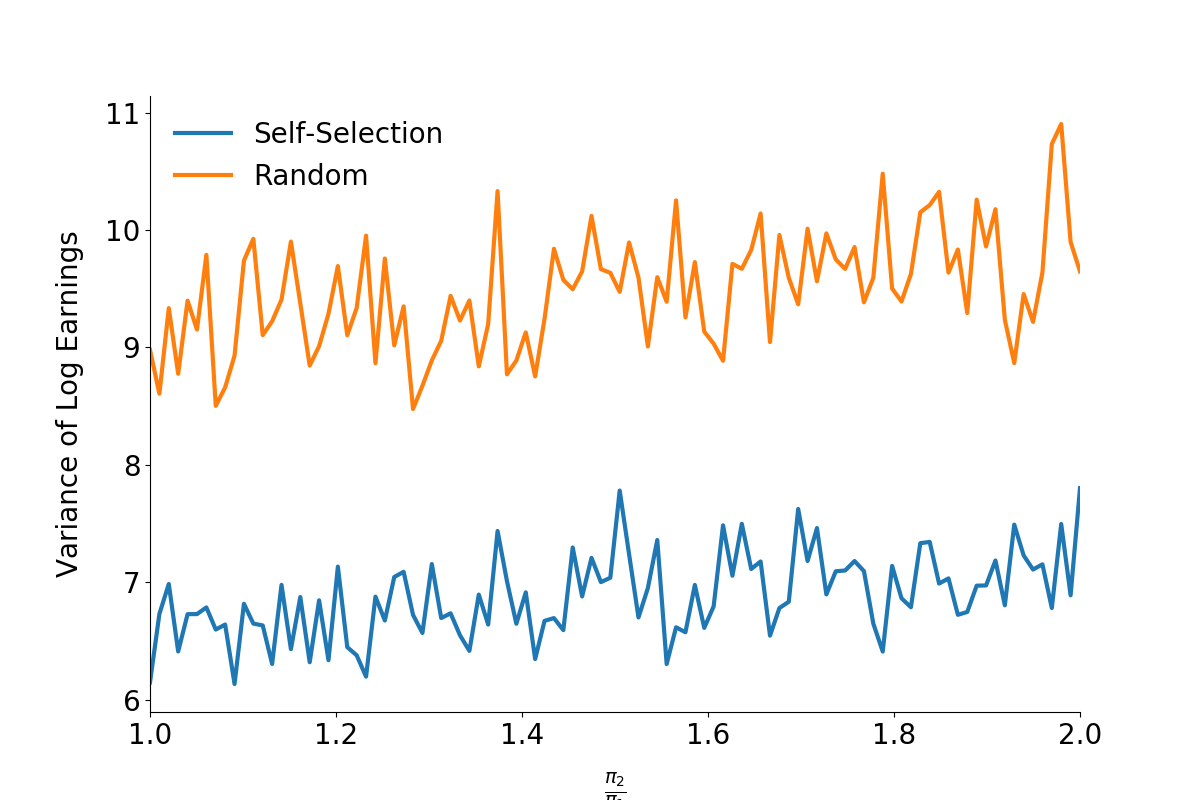
\includegraphics{fig-assignment-mechanism}}
	\end{center}
\end{frame}
%-------------------------------------------------------------------------------
%-------------------------------------------------------------------------------
\begin{frame}
	\begin{center}
		\LARGE\textit{Incarnations of the Roy Model}
	\end{center}
\end{frame}